\documentclass[runningheads]{llncs}
\usepackage[T1]{fontenc}
\usepackage{amsmath,amssymb,booktabs,graphicx,multirow}
\usepackage[hidelinks]{hyperref}
\begin{document}
\title{When Fewer Labels Are More Valuable: Learning under Risk Constraints and Delayed Feedback}
\titlerunning{When Fewer Labels Are More Valuable}
\author{Anonymous Authors}
\authorrunning{Anonymous Authors}
\institute{Anonymous Institution}
\maketitle
\begin{abstract}
Risk-constrained label acquisition couples learning with the actions that reveal outcomes. With delayed feedback, a feasible set containing more labels can be less valuable than a smaller set covering different information directions. We study this separation through a same-state quantity--composition decomposition and a two-direction information model that gives an explicit threshold for a pending-induced preference reversal. We also distinguish post-outcome acquisition opportunity from value achievable before labels arrive. These analyses lead to DC-PRISM, a policy that compares feasible sets with a quantity reference using pending-aware, target-weighted information. In 128 controlled worlds, DC-PRISM reduces mean Brier loss from 0.136683 to 0.120234 while selecting 3.266 rather than 6 labels. Fresh controlled comparisons confirm gains of the fixed-family rule over quantity and information references. Across 256 paired interventions on real covariates, coverage gaps enlarge post-outcome opportunity in three of four settings, while policy gains remain unconfirmed. Ten-round replay on four processed credit cohorts shows heterogeneous utility, including a confirmed 0.004139 ALC-Brier gain over fixed-count acquisition on PPDai. Together, the results connect the information geometry of feasible choices to both the benefits and the boundaries of adaptive acquisition.
\keywords{Selective labels \and Risk-constrained acquisition \and Delayed feedback \and Active learning}
\end{abstract}
\section{Introduction}
\label{sec:intro}

Label acquisition in decision systems changes both the training data and the system's exposure to adverse outcomes. A lender observes repayment after granting credit, while rejected applications remain unlabeled. This selective-label structure makes the data available for future learning depend on earlier decisions~\cite{lakkaraju2017selective,wei2021selective}. When outcomes arrive with a delay, the learner must also account for applications already accepted but not yet settled. The resulting acquisition problem combines a risk budget, incomplete coverage of the population, and information that is committed but still pending.

A risk budget determines which label sets are feasible, but feasible label count does not determine predictive value. Classical active learning and experimental design select observations by their expected contribution to estimation or prediction~\cite{cohn1996active,yu2006transductive}. More recent methods explicitly optimize Fisher-based estimation criteria, predictive information, or downstream loss~\cite{ash2021fishing,bickfordsmith2023prediction,huang2026loss}. These objectives make composition central: observations can differ in relevance to the target population and in redundancy with the existing data. Risk constraints add a further interaction because acquiring one informative but more exposed observation can displace several less exposed observations. Pending feedback changes the comparison again because information along particular directions is already scheduled to arrive.

We study this interaction through a reference question: when does a smaller risk-feasible set yield more learning value than a quantity-oriented reference? The reference holds the operational risk budget fixed and makes the quantity trade-off explicit. We first separate the realized predictive gain into a quantity term and a composition term, evaluated from the same information state. We then analyze a two-direction Gaussian information model. When pending information accumulates along the reference set's direction, the value of further observations in that direction falls, and an alternative set can become preferable at a calculable threshold. This analysis identifies the direction of pending information as a condition that changes the selection decision even when the feasible sets and budget stay fixed.

The mechanism's practical value depends on choosing a set before its labels arrive. We distinguish the best set after training outcomes are revealed from the best choice based on visible information. This separates foresight advantage from pre-outcome selection quality and explains why increased post-outcome opportunity can coexist with little policy gain.

These observations lead to DC-PRISM, a policy that compares risk-feasible candidate sets against the quantity reference using a target-weighted information proxy. It includes pending covariates, evaluates relative value with common parameter draws, charges for reductions in label count, and retains the reference when the score does not justify a change. In 128 original controlled worlds, DC-PRISM obtains mean Brier loss 0.120234, compared with 0.136683 for the risk reference, while acquiring fewer labels. Fresh controlled comparisons, 256 paired coverage interventions, and four-cohort delayed replay examine how these gains vary across information states and datasets.

Our contributions are:
\begin{itemize}
\item A mechanism analysis of risk-feasible quantity and predictive value, combining a same-state quantity--composition decomposition with an explicit condition for selection reversal under directional pending information.
\item A layered empirical study linking controlled gains, common-family comparisons, and coverage interventions, together with an ex ante versus post-outcome distinction that makes the opportunity diagnostics interpretable.
\item DC-PRISM, a mechanism-informed acquisition policy, evaluated through controlled comparisons and delayed replay on four processed credit cohorts with fixed budgets and legal feedback timing.
\end{itemize}


\section{Setting and Research Questions}
\label{sec:setting}

At round $t$, a learner observes labeled history $D_t$, covariates of pending acquisitions $O_t$, an unlabeled candidate pool $C_t$, and target covariates $Q_t$. Each candidate $i$ has a visible nonnegative exposure $e_i$ and an adverse binary outcome $Y_i$ revealed only after acquisition and its feedback delay. The information available when selecting a set is denoted by $\mathcal H_t$. A legal policy chooses $S_t\subseteq C_t$ using $\mathcal H_t$; outcomes in $O_t$ and $C_t$ remain hidden. Ordinary acquisitions enter the pending queue independently of the exploration policy. 

We evaluate learning with the Brier score, the mean squared error of probability predictions~\cite{brier1950verification}. For a fixed state, $L(S;Y)$ denotes the test loss after fitting on $D\cup O\cup S$, with $Y$ collecting the training outcomes that were hidden during selection. This post-settlement endpoint compares sets from the same state. Online evaluation instead uses only outcomes released by the start of each round. The two endpoints answer complementary questions about set value and delayed policy performance.

\paragraph{Risk-feasible acquisition.}
Let $q_i\in[0,1]$ be the risk score available at selection, $\ell=\log(1/\alpha)$, and
\begin{equation}
 \phi(q)=\begin{cases}q(1-q),&q\leq 1/2,\\1/4,&q>1/2.\end{cases}
\end{equation}
For nonempty $S$, define
\begin{equation}
\begin{split}
 \mu_U(S)&=\sum_{i\in S}e_iq_i,\qquad
 V_U(S)=\sum_{i\in S}e_i^2\phi(q_i),\\
 R_\alpha(S)&=\mu_U(S)+\sqrt{2V_U(S)\ell}
                  +\tfrac13\ell\max_{i\in S}e_i.
\end{split}\label{eq:envelope}
\end{equation}
Set $R_\alpha(\varnothing)=0$ and let
$\mathcal A_t=\{S\subseteq C_t:R_\alpha(S)\leq B_t\}$.
The envelope defines the operational feasible region through mean loss, dispersion, and maximum exposure.

The probability interpretation follows from a standard sub-gamma bound~\cite{boucheron2013concentration}. Conditional on $\mathcal H_t$, suppose the selected outcomes are independent Bernoulli variables with $p_i\leq q_i$. Their weighted sum $Z_S=\sum_{i\in S}e_iY_i$ has mean at most $\mu_U(S)$ and variance at most $V_U(S)$. With $m=\max_{i\in S}e_i$,
\begin{equation}
 \log\mathbb E\!\left[e^{\lambda(Z_S-\mathbb E Z_S)}\mid\mathcal H_t\right]
 \leq \frac{V_U(S)\lambda^2}{2(1-\lambda m/3)},
 \quad 0<\lambda<3/m.
\end{equation}
Chernoff optimization therefore gives
$\Pr\{Z_S>R_\alpha(S)\mid\mathcal H_t\}\leq\alpha$.
The experiments use empirical Wilson/Laplace risk scores; the bound applies when the stated simultaneous upper-coverage and independence conditions hold.

\paragraph{Quantity reference and questions.}
We construct a reference $M_K\in\mathcal A_t$ that prioritizes cardinality and breaks ties by smaller envelope. Enumeration solves this problem for small pools; larger pools use exposure-stratified feasible search and a cardinality upper bound. Here $K=|M_K|$ denotes the returned feasible count. Our questions are: (i) how do quantity and composition contribute to the gain over $M_K$; (ii) when does pending information reverse the preferred composition; and (iii) how much observed opportunity can a policy exploit before outcomes arrive? DC-PRISM addresses the third question by comparing candidate sets against $M_K$ using a target-weighted information score; Section~\ref{sec:policy} specifies the rule.

\section{Mechanism Analysis}
\label{sec:mechanism}

\subsection{Quantity and Composition}
For a selected set $S$ of size $k\leq K$, let $M_k$ be a feasible risk-ranked reference of size $k$, with $M_K$ reused when $k=K$. All three models start from the same $D\cup O$ and use the same realized outcomes. Define
\begin{equation}
\begin{split}
 Q_k&=L(M_k;Y)-L(M_K;Y),\\
 C_k&=L(M_k;Y)-L(S;Y),\\
 J&=L(M_K;Y)-L(S;Y)=C_k-Q_k.
\end{split}\label{eq:decomposition}
\end{equation}
The quantity term compares two risk references; the composition term compares equally sized sets. Positive $J$ means composition more than compensates for the quantity term. The sign of $Q_k$ depends on the fitted models and realized labels: a larger reference can have higher test loss.

Risk couples label count and information direction because one informative observation can displace several cheaper ones. Pending information adds substitution: a direction uncovered in $D$ may already be represented in $O$.

\subsection{Directional Pending Information}
Consider a two-parameter linear Gaussian model with precision
$H=\operatorname{diag}(h_1,h_2)$ and target weight
$G=\operatorname{diag}(g_1,g_2)$, all entries positive. The learning loss is weighted posterior predictive variance $\operatorname{tr}(GH^{-1})$. Pending observations add precision $o\geq0$ along direction 1. Two feasible actions are available: the quantity reference adds total precision $a>0$ along direction 1; a smaller alternative adds $b>0$ along direction 2. Their risk-feasible status is held fixed as $o$ varies.

\begin{proposition}[Directional preference reversal]
The gain from choosing the alternative rather than the quantity reference is
\begin{equation}
 J(o)=\frac{g_2b}{h_2(h_2+b)}
       -\frac{g_1a}{(h_1+o)(h_1+o+a)}.\label{eq:reversal}
\end{equation}
It is strictly increasing in $o$. Writing
$v_2=g_2b/[h_2(h_2+b)]$, the alternative is preferred exactly when
\begin{equation}
 o>o^*=\frac{-a+\sqrt{a^2+4g_1a/v_2}}{2}-h_1.\label{eq:threshold}
\end{equation}
A reversal within $o\geq0$ occurs when $o^*>0$.
\end{proposition}
\begin{proof}
The reference loss is $g_1/(h_1+o+a)+g_2/h_2$ and the alternative loss is $g_1/(h_1+o)+g_2/(h_2+b)$. Subtraction gives~\eqref{eq:reversal}. The derivative is
$g_1a[2(h_1+o)+a]/[(h_1+o)^2(h_1+o+a)^2]>0$.
Solving $(h_1+o)(h_1+o+a)>g_1a/v_2$ gives~\eqref{eq:threshold}.
\end{proof}

The reversal can occur under an unchanged exposure budget. Set $h_1=h_2=g_1=g_2=1$, and compare four unit-information labels on direction 1 with one on direction 2, so $a=4$ and $b=1$. With $\alpha=0.1$, common risk score $q=0.1$, and exposures $0.1$ for each reference label and approximately $0.16244812$ for the alternative, both actions have envelope $B\approx0.24551080$. Combining the alternative with even one reference item exceeds $B$. These exposure values specify the feasible actions independently of the Gaussian information model.

\begin{figure}[t]
 \centering
 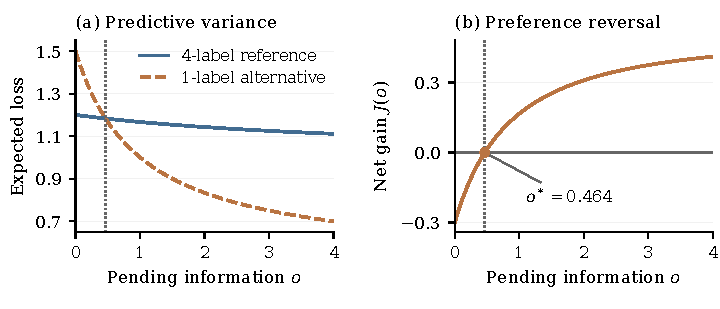
\includegraphics[width=\linewidth]{figures/fig_information_reversal.pdf}
 \caption{Analytical preference reversal in the two-direction Gaussian model. Both actions satisfy the same fixed risk budget. The one-label alternative becomes preferable at $o^*\approx0.464$ as pending information accumulates along the four-label reference direction. Loss is weighted posterior predictive variance.}
 \label{fig:reversal}
\end{figure}

At $o=0$, the reference and alternative losses are $1.2$ and $1.5$. At $o=1$, they are $1.166667$ and $1.0$, respectively. Figure~\ref{fig:reversal} shows the transition at $o^*\approx0.464102$. The mechanism is directional redundancy: pending information reduces the value of another observation on the reference axis while leaving the other axis's incremental value unchanged. The threshold describes this diagonal model and motivates evaluating candidates against history plus expected pending information.

\subsection{Opportunity Before and After Outcomes}
The best set after seeing training outcomes need not be the best decision before those outcomes arrive. Fix visible information $\mathcal H$ and a finite candidate family $\mathcal F$ containing reference $M$. Let $L(S,Y)$ average over test outcomes but retain the dependence on hidden training labels $Y$. Define
\begin{align}
 H_{\mathrm{post}}&=\mathbb E\!\left[L(M,Y)-\min_{S\in\mathcal F}L(S,Y)\mid\mathcal H\right],\label{eq:post}\\
 H_{\mathrm{pre}}&=\mathbb E[L(M,Y)\mid\mathcal H]
      -\min_{S\in\mathcal F}\mathbb E[L(S,Y)\mid\mathcal H].\label{eq:pre}
\end{align}
Because the expectation of a minimum is no larger than the minimum of expectations,
$H_{\mathrm{post}}\geq H_{\mathrm{pre}}\geq0$.
For any legal within-family policy with expected gain $G_\pi$,
\begin{equation}
 H_{\mathrm{post}}-G_\pi
  =\underbrace{H_{\mathrm{post}}-H_{\mathrm{pre}}}_{\text{foresight advantage}}
   +\underbrace{H_{\mathrm{pre}}-G_\pi}_{\text{pre-outcome selection gap}}.\label{eq:opportunity}
\end{equation}
The empirical family minimum measures opportunity conditional on realized training labels. It can increase while additional pre-outcome value stays small, a distinction used in the coverage intervention below.

\section{Controlled Evidence}
\label{sec:controlled}

\subsection{Controlled Selection Gains}
\paragraph{Design.}
Each synthetic world has six features, 80 historical labels, 22 pending acquisitions, 24 candidates, 180 target covariates, and 240 test observations. History has narrow coverage of the candidate directions. Candidate groups contain low-risk core observations, observations aligned with the pending direction, observations along two other predictive directions, and auxiliary-tail observations. Exposure ranges vary by group. Pending observations concentrate on the second feature direction; the target distribution also covers the third and fourth directions. Outcomes are drawn from a fixed Bernoulli model with a logistic core and piecewise auxiliary-tail effects. This design supplies both redundant and complementary feasible acquisitions.

All set choices use the same history, candidate pool, risk scores and numerical budget within a world. Labels are used for evaluation after selections are fixed. We first analyze 128 original worlds, then use 128 fresh worlds for common-family comparisons. The second study also includes four real-covariate settings with generated outcomes, giving 35 registered primary comparisons overall. We report paired mean differences with 95 percent Bonferroni simultaneous $t$ intervals and Holm-adjusted tests~\cite{holm1979simple}. A gain is materially positive when its simultaneous lower endpoint exceeds $10^{-4}$ Brier. World counts and comparison families were fixed before these batches ran.

\begin{table}[t]
\caption{Post-settlement Brier and mean acquisition count in two batches of 128 controlled worlds. The original fixed-count row uses the repaired four-label rule; the fresh fixed-count row uses five labels and common-family point-value selection. DC-PRISM retains its full search in both batches.}
\label{tab:controlled}
\centering
\small
\begin{tabular}{lrrrr}
\toprule
& \multicolumn{2}{c}{Original worlds} & \multicolumn{2}{c}{Fresh worlds} \\
\cmidrule(lr){2-3}\cmidrule(lr){4-5}
Policy & Brier $\downarrow$ & Labels & Brier $\downarrow$ & Labels \\
\midrule
Safe-MinRisk & 0.136683 & 6.000 & 0.147046 & 6.000 \\
Fixed count & 0.136720 & 4.000 & 0.141038 & 5.000 \\
Fisher-cost & 0.143776 & 2.719 & 0.153765 & 2.680 \\
DC-PRISM & 0.120234 & 3.266 & 0.130807 & 3.203 \\
Common-family Full & -- & -- & 0.134644 & 4.352 \\
\bottomrule
\end{tabular}
\end{table}


\paragraph{Quantity and composition in realized learning.}
DC-PRISM improves Brier loss while selecting fewer labels in both controlled batches (Table~\ref{tab:controlled}). In the original worlds, its mean loss is $0.120234$, compared with $0.136683$ for Safe-MinRisk, with mean counts $3.266$ and $6$. The repaired fixed-count rule attains its four-label target and has loss $0.136720$; its paired excess loss over DC-PRISM is $0.016486$, with pointwise 95 percent interval $[0.010972,0.022001]$.

The same-state decomposition gives mean $C_k=0.016262$, $Q_k=-0.000187$, and $J=0.016449$ for DC-PRISM. The dominant term is the improvement from replacing the risk-ranked set with a different set at the selected cardinality. The small negative quantity term means the smaller risk reference itself performs slightly better in these realized fits. This result connects the observed gain to composition without presuming a cost from every reduction in count.

\paragraph{Common-family comparisons.}
To compare scoring components on the same alternatives, we construct a family without pending information and add feasible prefixes of $M_K$ at every cardinality. We then rescore this family under 16 combinations of pending information, lower versus upper quantile, quantity penalty, and fallback gate. We call the complete configuration \emph{Full}. Full, fixed count and the scoring controls share this family; Fisher-cost uses its own packing rule under the same state, risk scores and budget. DC-PRISM retains its full search. The common-family fixed-count rule maximizes point-value at size $\lceil0.75K\rceil$.

In the fresh controlled worlds, Full has mean Brier $0.134644$ and mean count $4.352$. Its gains over fixed count, Safe-MinRisk, and Fisher-cost are respectively $0.006394$, $0.012402$, and $0.019121$; all three simultaneous intervals exceed the material threshold (Figure~\ref{fig:controlled}). DC-PRISM's full search gives descriptive mean loss $0.130807$ with $3.203$ labels. 

\begin{figure}[t]
 \centering
 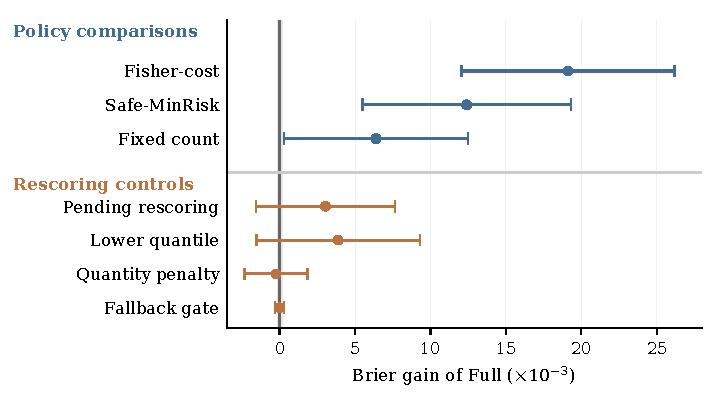
\includegraphics[width=\linewidth]{figures/fig_controlled_effects.pdf}
 \caption{Full in 128 fresh controlled worlds: comparator-minus-Full Brier with 95 percent simultaneous intervals over 35 comparisons. Scoring controls and fixed count share Full's family; Fisher-cost uses its own packing rule. Gray band: $\pm10^{-4}$ Brier.}
 \label{fig:controlled}
\end{figure}

The individual scoring contrasts are less decisive than the policy comparisons. Lower-quantile and pending-rescoring gains have positive means, $0.003885$ and $0.003044$, but their simultaneous intervals cross zero. Gate and quantity-penalty means are $-0.000007$ and $-0.000238$, also with intervals crossing zero. These results establish gains for the complete choice rule in this controlled regime while leaving the four isolated component effects unresolved.

\subsection{History Coverage and Opportunity}
\paragraph{Bridge to real covariates.}
We retain the observed covariates of HMEQ and LendingClub and generate labels from either
$p(x)=\sigma(-0.8+x^\top\beta)$, where
$\beta=(0.45,0.65,-0.5,0.35,0.2,-0.15)$,
or a nonlinear logit adding $0.5\sin(x_2)+0.35x_3x_4$.
Each of the four settings contains 64 worlds. Median imputation and scaling are fitted on the historical sample; the auxiliary coordinates are retained without tail-hinge transformation. Common-family Full's mean gains over Safe-MinRisk range from $-0.000038$ to $0.000036$, with no material advantage established. Mean post-outcome family headroom falls from approximately $0.0205$ in the controlled generator to $0.0016$--$0.0018$ in these settings.

\paragraph{Paired coverage intervention.}
We next change history while fixing the reference decision problem. Within each new world, a reservoir contains 240 randomly sampled records. The broad arm uses the first 80; the gap arm uses the 80 lowest values of the second transformed feature. Candidate, pending, target and test records, their generated labels, preprocessing, risk scores, numerical budget, reference, and candidate family are identical across arms. Preprocessing and the risk/family construction use the broad reference history once, while the predictive learner is fitted to each arm's history. The intervention therefore isolates history coverage conditional on that frozen reference problem.

The study contains another 64 paired worlds per setting, or 256 pairs. Its primary endpoint is expected Brier on the fixed test covariates,
\begin{equation}
 L_p(S;Y)=\frac1{|T|}\sum_{j\in T}
 \big[(\widehat p_{S,j}-p_j)^2+p_j(1-p_j)\big],\label{eq:expectedbrier}
\end{equation}
which integrates test-label randomness while preserving the realized training outcomes. The 16 primary comparisons form a separate simultaneous-inference family.

\begin{figure}[t]
 \centering
 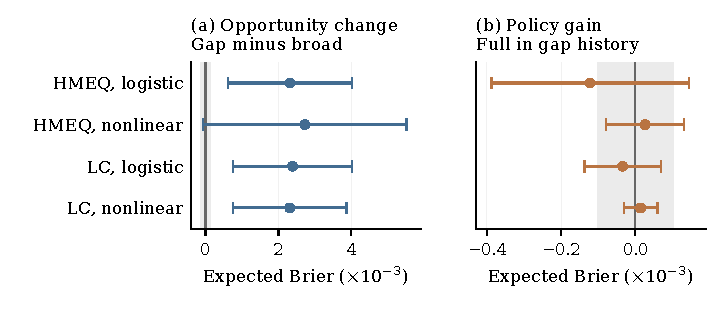
\includegraphics[width=\linewidth]{figures/fig_coverage_opportunity.pdf}
 \caption{Coverage intervention, with 64 paired worlds per setting. Left: change in post-outcome family headroom from broad to gap history. Right: Full's gain over the risk reference in gap history. Bars are 95 percent simultaneous intervals from the 16-comparison family. Axes have different scales; gray bands are $\pm10^{-4}$ expected Brier. LC denotes LendingClub.}
 \label{fig:coverage}
\end{figure}

Coverage gaps increase post-outcome headroom in three settings by $0.002320$, $0.002391$, and $0.002312$, with simultaneous lower endpoints $0.000622$, $0.000756$, and $0.000753$ (Figure~\ref{fig:coverage}). HMEQ with nonlinear outcomes has mean increase $0.002726$ and interval $[-0.000061,0.005513]$. Full's gain in the gap arm remains unconfirmed in all four settings; the LendingClub nonlinear interval lies entirely within $\pm10^{-4}$.

History coverage changes which realized sets perform best, while Full yields little gain over the risk reference. Equation~\eqref{eq:opportunity} separates foresight about hidden training labels from imperfect pre-outcome selection; the saved family minima measure their combined effect.

\section{A Mechanism-Informed Acquisition Strategy}
\label{sec:policy}

\subsection{Target-Weighted Information}
DC-PRISM approximates the incremental value of a feasible set after pending acquisitions settle. We fit an $\ell_2$-regularized logistic model on $D$ and write $\bar x=(1,x^\top)^\top$, $p_\theta(x)=\sigma(\bar x^\top\theta)$, and $w_\theta(x)=p_\theta(x)[1-p_\theta(x)]$. The information and target matrices are
\begin{align}
 H_{D+O}(\theta)&=\Lambda+\sum_{i\in D\cup O}w_\theta(x_i)\bar x_i\bar x_i^\top,\\
 G_Q(\theta)&=\frac1{|Q|}\sum_{j\in Q}w_\theta(x_j)^2\bar x_j\bar x_j^\top,\\
 A_S(\theta)&=\sum_{i\in S}w_\theta(x_i)\bar x_i\bar x_i^\top.
\end{align}
The matrix $G_Q$ weights parameter uncertainty by the sensitivity of target predictions. The resulting local quadratic Brier-reduction proxy is
\begin{equation}
 V_\theta(S)=\operatorname{tr}\!\left[
 G_Q(\theta)\{H_{D+O}(\theta)^{-1}
       -(H_{D+O}(\theta)+A_S(\theta))^{-1}\}\right].\label{eq:value}
\end{equation}
This target weighting follows the predictive focus of experimental design~\cite{yu2006transductive} and information-based acquisition~\cite{ash2021fishing,bickfordsmith2023prediction}. Pending covariates enter the information matrix without revealing their labels. In the two-direction model, this is the operation that discounts an already-covered direction.

\subsection{Selection Relative to a Feasible Reference}
The candidate family contains $M_K$, feasible prefixes constructed by marginal utility per marginal envelope cost, value-ranked prefixes, and exchanges retaining part of $M_K$ before packing other candidates. Conservative and optimistic curvature rankings add alternative directions to the search. Each proposal is checked against~\eqref{eq:envelope}. Enumeration cutoffs are 16 candidates in controlled studies and 14 in replay; larger pools use stratified prefix search, local exchanges and a count upper bound. A closed bound certifies the reference count, while the risk tie break remains heuristic.

Shared parameter draws compare the proposed sets under common model uncertainty. Draw $\theta^{(m)}\sim\mathcal N(\widehat\theta,H_D^{-1})$ using the local Gaussian approximation~\cite{mackay1992practical}. For candidate information, use damped curvature
\begin{equation}
 \widetilde w_i^{(m)}=w_{\theta^{(m)}}(x_i)
 \exp\!\left[-0.45\{\bar x_i^\top(\theta^{(m)}-\widehat\theta)\}^2\right].
\end{equation}
Let $\widetilde V_m$ denote~\eqref{eq:value} with draw-specific matrices and candidate curvatures floored at $10^{-6}$. Set $a_m=\max\{\widetilde V_m(M_K),10^{-6}\}$ and define
\begin{align}
 d_m(S)&=\tanh\!\left(
 \frac{\widetilde V_m(S)-a_m}{2.5a_m}\right),\\
 Z(S)&=\widehat{\operatorname{quantile}}_{0.2}\{d_m(S)\}
       -0.22\frac{(K-|S|)_+}{\max(K,1)}.\label{eq:score}
\end{align}
Choose the maximizer of $Z$ if its score exceeds $0.08$; otherwise choose $M_K$. The empirical quantile summarizes parameter uncertainty; the penalty and gate require a lower-count choice to improve sufficiently on the reference.

To construct $q$, we compute a one-sided Wilson upper rate ($z=1.645$) on the upper half of fitted historical risks. We clip this rate between their mean fitted risk and $0.98$, take the logit difference from that mean, and clip the shift to $[0.15,1.15]$. We add that shift to 40 Laplace-draw logits, take their $0.9875$ quantile, apply the sigmoid, and clip to $[10^{-6},0.999]$. These risk draws are separate from the utility draws. For $F$ proposed sets, $M$ draws and $d$ model parameters, the matrix inversions in scoring cost $O(MFd^3)$, with draw matrices reused across sets. The experiments use six features plus intercept, slope regularization $0.45$, and intercept ridge $10^{-4}$ in the information matrices. There are 20 parameter draws in the controlled studies and 16 in online replay. All scoring parameters remain fixed in the fresh replay.

\section{Real-Cohort Replay}
\label{sec:replay}

\subsection{Data and Delayed Protocol}
We use a fixed supplied archive of six-feature processed cohorts labeled HMEQ, LendingClub, PPDai and UCI Credit (Table~\ref{tab:data}). HMEQ home-equity data, LendingClub loan records and UCI credit-default data provide the corresponding application sources~\cite{sasHMEQ,lendingclubSource,yeh2009comparison}. The replay uses the archive's recorded binary outcomes and exposure fields. Cohort labels identify these supplied processed inputs; all reported sample sizes and feature counts refer to that archive.

\begin{table}[t]
\caption{Supplied processed cohorts used in the replay, each with six input features and binary recorded outcomes. Exposure is normalized using the initial history before entering the acquisition constraint.}
\label{tab:data}
\centering
\small
\begin{tabular}{lrrl}
\toprule
Cohort & Rows & Positive labels (percent) & Exposure field \\
\midrule
HMEQ & 5,960 & 19.95 & Loan amount \\
LendingClub & 10,624 & 20.70 & Loan principal \\
PPDai & 55,596 & 12.92 & Credit limit \\
UCI Credit & 30,000 & 22.12 & Credit-card limit \\
\bottomrule
\end{tabular}
\end{table}


For each cohort and seed, we reserve 1,000 test rows, 600 unlabeled target rows and a disjoint 600-row historical reservoir. A covariate-ranked rule selects 68 initial historical records. The remaining records form a constructed stream: each round has 24 candidates and 14 ordinary acquisitions selected through observable feature and exposure ranks, then randomized within the designated groups. The stream supplies low-risk, pending-aligned, complementary, and tail observations. Sixteen fresh random split/stream seeds are used for each cohort. The evaluation is therefore conditional on the four fixed cohorts and the specified stream construction.

Preprocessing is fitted on the initial 68 records. It imputes medians, standardizes and clips features at $\pm4.5$, and applies a tail hinge to the last two coordinates. Hinge thresholds use the initial-history 90th percentiles with floor $1.35$ and scale $1.85$. Exposure is winsorized at the initial 5th and 95th percentiles and divided by its winsorized mean. The numerical budget is fixed across policies using the initial reference model: it is $1.03$ times the envelope of six candidates ranked by a common risk/dispersion score. During replay, each policy updates its own learner and empirical $q$ from its released outcomes.

Exploration labels arrive one round after selection, while ordinary labels arrive two rounds later. At each round's start, due outcomes are released and Brier loss is measured before the new acquisitions reveal any labels. The pending state contains the unreleased queue and the current ordinary acquisitions. The primary metric is
\begin{equation}
 \mathrm{ALC\text{-}Brier}=\frac1{10}\sum_{t=1}^{10}
 \frac1{|T|}\sum_{j\in T}(Y_j-\widehat p_{t,j})^2.
\end{equation}
Methods share the initial data, external stream, target/test sets, budget sequence, model class and feedback timing. Their subsequent histories differ according to their acquisitions.

We compare DC-PRISM with four references. \emph{Ordinary only} acquires no additional labels. \emph{Safe-MinRisk} selects the feasible quantity reference. \emph{Fixed count} targets $\lceil0.75K\rceil$ labels using point-value/cost ranking and falls back to an anchor subset if greedy packing misses that count. \emph{Fisher-cost} ranks the single-observation reduction in unweighted parameter variance, using $G=I$, divided by an exposure-risk cost; it greedily packs feasible candidates without updating that initial ranking. This is the implemented Fisher-based comparator. Three comparisons per cohort---Safe-MinRisk, fixed count and Fisher-cost---form the 12-test primary family. Tests pair methods by seed; simultaneous intervals and the $10^{-4}$ material threshold follow the controlled-study convention.

\subsection{Online Results}
\begin{table}[t]
\caption{Ten-round replay on four supplied credit cohorts. ALC averages the Brier scores measured after due feedback arrives and before current-round selection. Standard deviations describe split/stream variation. Policy histories evolve separately under shared streams and numerical budgets.}
\label{tab:replay}
\centering
\small
\begin{tabular}{lrrrr}
\toprule
Policy & HMEQ & LendingClub & PPDai & UCI Credit \\
\midrule
\multicolumn{5}{l}{Mean online ALC-Brier $\downarrow$ (standard deviation across 16 seeds)} \\
Ordinary only & 0.1733 (0.0317) & 0.1672 (0.0143) & 0.1398 (0.0244) & 0.1731 (0.0224) \\
Safe-MinRisk & 0.1723 (0.0312) & 0.1666 (0.0134) & 0.1351 (0.0161) & 0.1725 (0.0228) \\
Fixed count & 0.1719 (0.0314) & 0.1666 (0.0137) & 0.1331 (0.0129) & 0.1724 (0.0230) \\
Fisher-cost & 0.1654 (0.0273) & 0.1653 (0.0135) & 0.1306 (0.0122) & 0.1719 (0.0256) \\
DC-PRISM & 0.1687 (0.0330) & 0.1657 (0.0100) & 0.1290 (0.0117) & 0.1724 (0.0244) \\
\midrule
\multicolumn{5}{l}{Mean selected labels per round} \\
Safe-MinRisk & 6.537 & 6.319 & 6.844 & 7.444 \\
Fixed count & 5.362 & 5.256 & 5.556 & 6.000 \\
Fisher-cost & 3.125 & 3.119 & 3.825 & 5.344 \\
DC-PRISM & 4.319 & 3.900 & 5.419 & 6.638 \\
\bottomrule
\end{tabular}
\end{table}


The online results vary across cohorts (Table~\ref{tab:replay}). DC-PRISM's mean ALC-Brier is lower than Safe-MinRisk on all four, with gains from $0.000124$ on UCI Credit to $0.006090$ on PPDai. Its mean is lower than fixed count on HMEQ, LendingClub and PPDai, and nearly equal on UCI Credit. Fisher-cost has lower mean loss on HMEQ, LendingClub and UCI Credit; DC-PRISM has lower mean loss on PPDai.

The primary simultaneous intervals identify one material positive comparison: DC-PRISM improves over fixed count on PPDai by $0.004139$, with interval $[0.000518,0.007759]$ and Holm-adjusted $p=0.018599$. The other 11 intervals include zero (Table~\ref{tab:replay_intervals}). Thus the replay supports a cohort-specific improvement while retaining uncertainty about the remaining pairwise effects.

\begin{table}[t]
\caption{Primary paired gains of DC-PRISM in online ALC-Brier, in units of $10^{-3}$. Positive gain favors DC-PRISM. Intervals are 95 percent simultaneous Bonferroni intervals across all 12 comparisons; the material threshold is $0.1$ in these units.}
\label{tab:replay_intervals}
\centering
\small
\begin{tabular}{llrr}
\toprule
Cohort & Comparator & Gain $\uparrow$ & Simultaneous interval \\
\midrule
HMEQ & Safe-MinRisk & +3.624 & [-3.219, +10.468] \\
 & Fixed count & +3.256 & [-3.477, +9.989] \\
 & Fisher-cost & -3.288 & [-11.100, +4.524] \\
\addlinespace
LendingClub & Safe-MinRisk & +0.945 & [-3.632, +5.523] \\
 & Fixed count & +0.939 & [-3.931, +5.809] \\
 & Fisher-cost & -0.416 & [-5.681, +4.849] \\
\addlinespace
PPDai & Safe-MinRisk & +6.090 & [-0.834, +13.014] \\
 & Fixed count & +4.139 & [+0.518, +7.759] \\
 & Fisher-cost & +1.605 & [-1.002, +4.212] \\
\addlinespace
UCI Credit & Safe-MinRisk & +0.124 & [-2.362, +2.610] \\
 & Fixed count & -0.028 & [-2.471, +2.415] \\
 & Fisher-cost & -0.464 & [-2.739, +1.811] \\
\bottomrule
\end{tabular}
\end{table}


Acquisition counts help interpret these differences. DC-PRISM selects fewer labels per round than Safe-MinRisk in every cohort, but the reduction varies from $0.806$ on UCI Credit to $2.419$ on LendingClub. Its PPDai count, $5.419$, is close to fixed count's $5.556$, while their mean predictive losses differ by $0.004139$. On HMEQ, Fisher-cost selects $3.125$ labels compared with DC-PRISM's $4.319$ and has lower mean loss. Both patterns reinforce the need to examine composition alongside quantity.

Risk-envelope utilization for DC-PRISM averages $0.964$--$0.978$ across cohorts. The four nonempty envelope-constrained methods have zero recorded envelope violations and zero realized budget exceedances in these runs. These are replay frequencies under normalized exposure. Timing, disjointness and fixed-count checks pass for all 6,400 round records; replaying 80 trajectories reproduces the 800 checked rows exactly.

Controlled comparisons isolate set choices at a common state; online replay evaluates acquisition together with delayed updates and evolving estimates. Their differing results locate the practical challenge: translating a favorable feasible composition into a beneficial sequence of decisions.
\section{Related Work}
\label{sec:related}

\paragraph{Prediction-oriented and batch acquisition.}
Statistical active learning selects observations to improve a predictive model~\cite{cohn1996active}. Transductive experimental design incorporates the unlabeled target population into the selection criterion~\cite{yu2006transductive}; BAIT uses Fisher embeddings to optimize a bound on maximum-likelihood estimation error~\cite{ash2021fishing}. EPIG measures information gain in predictions~\cite{bickfordsmith2023prediction}, and loss-driven Bayesian active learning derives acquisition objectives from the downstream decision loss~\cite{huang2026loss}. BatchBALD accounts for dependencies among simultaneously acquired labels through joint mutual information~\cite{kirsch2019batchbald}. These works establish the predictive and geometric foundations used here. Our analysis concerns how an exposure-based feasible region interacts with pending information to change the relative value of quantity and composition. Fisher-cost implements the static trace-per-cost comparison defined in Section~\ref{sec:replay}.

\paragraph{Costs, selective labels, and delayed feedback.}
Cost-sensitive active learning studies the allocation of heterogeneous annotation effort~\cite{tomanek2010cost}, while ConBatch-BAL constructs batches under budget constraints~\cite{morato2025conbatch}. In decision systems, the cost of acquiring a label can instead arise from the action that reveals it. Selective-label research formalizes the resulting observation problem~\cite{lakkaraju2017selective}; Wei studies policies balancing learning cost against future utility~\cite{wei2021selective}, and Keswani et al. combine exploration with bounds on false-positive fractions and group coverage~\cite{keswani2024partial}. Active learning with logged data uses historical observations to guide further experimentation~\cite{yan2018logged}. Pham et al. account for verification latency by simulating the training data available when queried labels arrive~\cite{pham2022latency}. Our decision state includes both ordinary pending outcomes and earlier exploration outcomes. Holding this state and the risk budget fixed permits direct comparison of alternative feasible compositions.

\paragraph{Statistical foundations and credit prediction.}
The matrix proxy and parameter perturbations build on local Gaussian approximations used in Bayesian learning~\cite{mackay1992practical}. The risk envelope follows a sub-gamma concentration construction~\cite{boucheron2013concentration}; the empirical risk scores combine a Wilson adjustment~\cite{wilson1927probable} with parameter-draw quantiles. Predictive evaluation uses the Brier score~\cite{brier1950verification}, and the registered comparison families use Holm-adjusted tests~\cite{holm1979simple} alongside simultaneous intervals. Credit-default probability estimation provides a natural application of these distinctions~\cite{yeh2009comparison}. Our comparisons jointly specify target covariates, historical coverage, exposure constraints and future-label visibility to distinguish realized set value from pre-outcome decision value.

\section{Conclusion}
Risk-constrained label acquisition requires comparing the information supplied by feasible sets, including information already pending. A same-state quantity--composition decomposition makes this trade-off explicit, and a two-direction model gives a threshold at which pending information makes a smaller alternative preferable. Controlled studies demonstrate substantial gains with fewer acquisitions, while the coverage intervention separates post-outcome opportunity from improvement achieved by the selection rule. DC-PRISM turns these ideas into a policy based on a feasible reference and yields heterogeneous gains in delayed credit-cohort replay. The resulting research direction is to estimate pre-outcome learning value more directly, so that favorable information geometry can be converted into reliable acquisition decisions.

\clearpage
\bibliographystyle{splncs04}
\bibliography{refs}
\end{document}
